\documentclass[tikz,border=7pt]{standalone}

\usepackage[T1]{fontenc}
\usepackage{lmodern}
\usepackage{xcolor}
\usetikzlibrary{arrows.meta,calc,positioning}

% -----------------------------------------------------------------------------
% Apertus Difference Ranker: end-to-end experimental paradigm
% Compile with: pdflatex paradigm_tikz.tex
% -----------------------------------------------------------------------------

\definecolor{ink}{HTML}{12263A}
\definecolor{muted}{HTML}{52697D}
\definecolor{line}{HTML}{C9D7E2}
\definecolor{blue}{HTML}{1769AA}
\definecolor{blueLight}{HTML}{EAF4FB}
\definecolor{purple}{HTML}{7E57C2}
\definecolor{purpleLight}{HTML}{F0ECFB}
\definecolor{teal}{HTML}{159A8C}
\definecolor{tealLight}{HTML}{E8F7F4}
\definecolor{orange}{HTML}{E49A24}
\definecolor{orangeLight}{HTML}{FFF7E8}
\definecolor{panel}{HTML}{F8FAFC}

\tikzset{
  >={Latex[length=2.2mm]},
  flow/.style={->, draw=muted, line width=.8pt},
  blueflow/.style={->, draw=blue, line width=1.0pt},
  purpleflow/.style={->, draw=purple, line width=1.0pt},
  tealflow/.style={->, draw=teal, line width=1.0pt},
  orangeflow/.style={->, draw=orange, line width=1.0pt},
  panelbox/.style={rounded corners=3mm, draw=line, fill=panel, line width=.65pt},
  card/.style={rounded corners=2mm, draw=line, fill=white, line width=.65pt,
               align=center, inner sep=2.2mm, minimum height=.78cm,
               font=\small, text=ink},
  stage/.style={font=\bfseries\scriptsize, text=blue, align=center},
  heading/.style={font=\bfseries\small, text=ink, align=center},
  body/.style={font=\scriptsize, text=muted, align=center},
  pill/.style={rounded corners=1.6mm, draw=line, fill=white, inner sep=1.3mm,
               font=\bfseries\scriptsize, text=ink, align=center}
}

\begin{document}
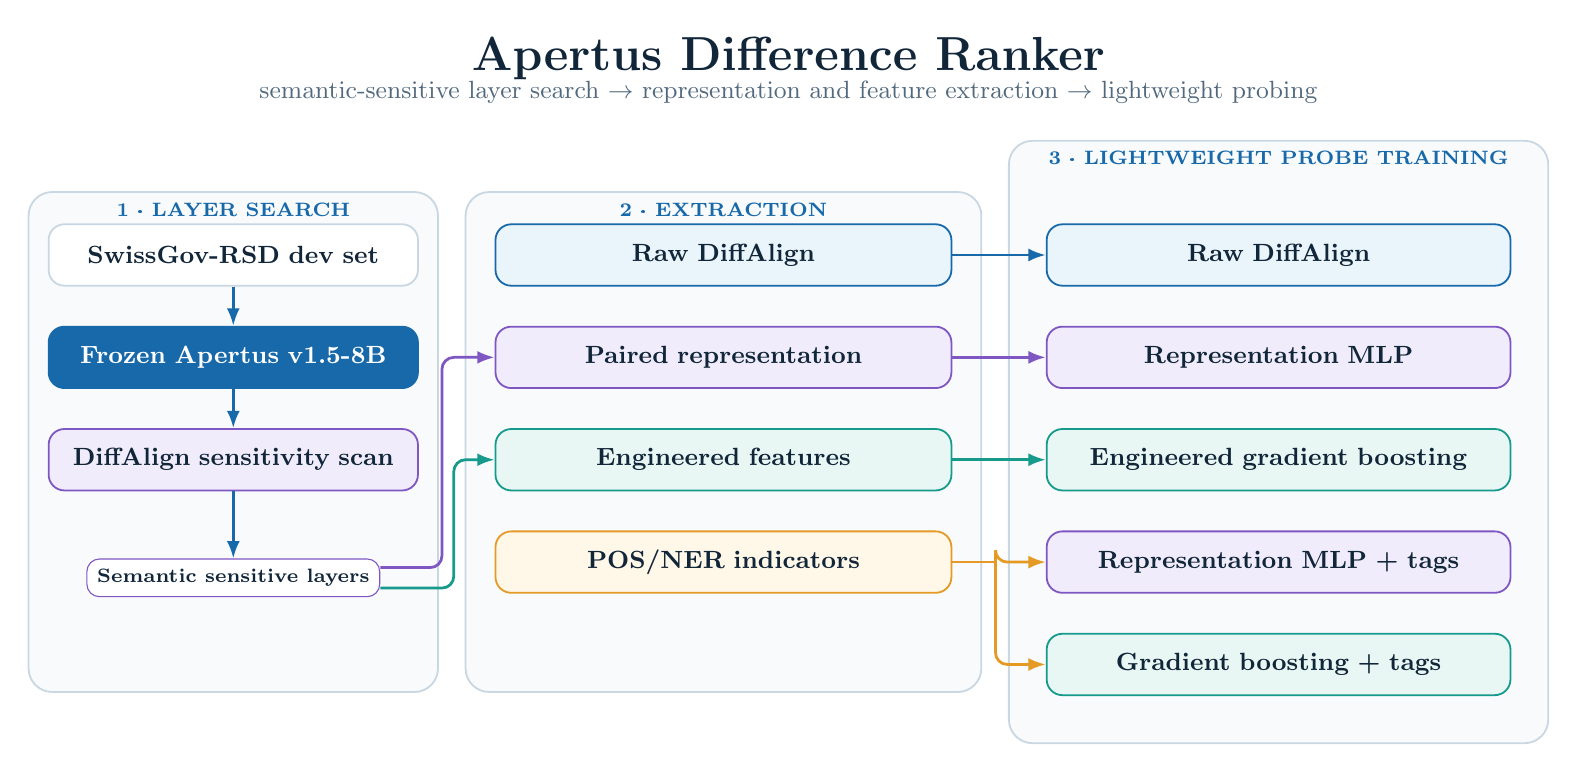
\begin{tikzpicture}[x=1cm,y=1cm]

  % Title
  \node[font=\bfseries\LARGE,text=ink] at (9.65,1.05)
    {Apertus Difference Ranker};
  \node[font=\small,text=muted] at (9.65,.62)
    {semantic-sensitive layer search $\rightarrow$ representation and feature extraction
     $\rightarrow$ lightweight probing};

  % Three main stage panels
  \draw[panelbox] (0,-.65) rectangle (5.20,-7.00);
  \draw[panelbox] (5.55,-.65) rectangle (12.10,-7.00);
  \draw[panelbox] (12.45,0) rectangle (19.30,-7.65);

  % ---------------------------------------------------------------------------
  % Stage 1
  % ---------------------------------------------------------------------------
  \node[stage,text width=4.65cm] at (2.60,-.88)
    {1 · LAYER SEARCH};

  \node[card,text width=4.25cm] (dev) at (2.60,-1.45) {
    \textbf{SwissGov-RSD dev set}
  };

  \node[card,text width=4.25cm,fill=blue,text=white,draw=blue]
    (apertus) at (2.60,-2.75) {
    \textbf{Frozen Apertus v1.5-8B}
  };

  \node[card,text width=4.25cm,fill=purpleLight,draw=purple]
    (scan) at (2.60,-4.05) {
    \textbf{DiffAlign sensitivity scan}
  };

  \node[pill,minimum width=3.6cm,draw=purple] (semanticlayers) at (2.60,-5.55)
    {Semantic sensitive layers};

  \draw[blueflow] (dev) -- (apertus);
  \draw[blueflow] (apertus) -- (scan);
  \draw[blueflow] (scan) -- (semanticlayers);

  % ---------------------------------------------------------------------------
  % Stage 2
  % ---------------------------------------------------------------------------
  \node[stage,text width=5.9cm] at (8.825,-.88)
    {2 · EXTRACTION};

  \node[card,text width=5.35cm,fill=blueLight,draw=blue]
    (raw) at (8.825,-1.45) {
    \textbf{Raw DiffAlign}
  };

  \node[card,text width=5.35cm,fill=purpleLight,draw=purple]
    (rep) at (8.825,-2.75) {
    \textbf{Paired representation}
  };

  \node[card,text width=5.35cm,fill=tealLight,draw=teal]
    (feat) at (8.825,-4.05) {
    \textbf{Engineered features}
  };

  \node[card,text width=5.35cm,fill=orangeLight,draw=orange]
    (ling) at (8.825,-5.35) {
    \textbf{POS/NER indicators}
  };

  % Parallel routes keep the two outputs visually aligned in the panel gap.
  \draw[purpleflow,rounded corners=1.5mm]
    ([yshift=1.3mm]semanticlayers.east) -- (5.25,-5.42) |- (rep.west);
  \draw[tealflow,rounded corners=1.5mm]
    ([yshift=-1.3mm]semanticlayers.east) -- (5.40,-5.68) |- (feat.west);

  % ---------------------------------------------------------------------------
  % Stage 3
  % ---------------------------------------------------------------------------
  \node[stage,text width=6.1cm] at (15.875,-.22)
    {3 · LIGHTWEIGHT PROBE TRAINING};

  \node[card,text width=5.45cm,fill=blueLight,draw=blue]
    (p0) at (15.875,-1.45) {
    \textbf{Raw DiffAlign}
  };
  \node[card,text width=5.45cm,fill=purpleLight,draw=purple]
    (p1) at (15.875,-2.75) {
    \textbf{Representation MLP}
  };
  \node[card,text width=5.45cm,fill=tealLight,draw=teal]
    (p2) at (15.875,-4.05) {
    \textbf{Engineered gradient boosting}
  };
  \node[card,text width=5.45cm,fill=purpleLight,draw=purple]
    (p3) at (15.875,-5.35) {
    \textbf{Representation MLP + tags}
  };
  \node[card,text width=5.45cm,fill=tealLight,draw=teal]
    (p4) at (15.875,-6.65) {
    \textbf{Gradient boosting + tags}
  };

  \draw[blueflow] (raw.east) -- (p0.west);
  \draw[purpleflow] (rep.east) -- (p1.west);
  \draw[tealflow] (feat.east) -- (p2.west);

  % One explicit POS/NER fork avoids overlapping duplicate arrow segments.
  \coordinate (lingfork) at (12.28,-5.35);
  \draw[draw=orange,line width=1.0pt] (ling.east) -- (lingfork);
  \draw[orangeflow,rounded corners=1.5mm] (lingfork) |- (p3.west);
  \draw[orangeflow,rounded corners=1.5mm] (lingfork) |- (p4.west);

\end{tikzpicture}
\end{document}
